\documentclass[11pt,letterpaper]{article}

\newenvironment{proof}{\noindent{\bf Proof:}}{\qed\bigskip}

\newtheorem{theorem}{Theorem}
\newtheorem{corollary}{Corollary}
\newtheorem{lemma}{Lemma} 
\newtheorem{claim}{Claim}
\newtheorem{fact}{Fact}
\newtheorem{definition}{Definition}
\newtheorem{assumption}{Assumption}
\newtheorem{observation}{Observation}
\newtheorem{example}{Example}
\newcommand{\qed}{\rule{7pt}{7pt}}

\newcommand{\assignment}[5]{
\thispagestyle{plain} 
\newpage
\setcounter{page}{1}
\noindent
\begin{center}
\framebox{ \vbox{ \hbox to 6.28in
{\bf \textsf{ #1 \hfill #2 }}
\vspace{4mm}
\hbox to 6.28in
{\hspace{2.5in}\Large\mbox{\bf \textsf{Problem Set #3}}}
\vspace{4mm}
\hbox to 6.28in
{{\it Handed Out: #4 \hfill Due: #5}}
}}
\end{center}
}
%\assignment{CS224W: Social and Information Network Analysis}{Fall 2012}{$1$}{September $11^{th}$, $2012$}{September $20^{th}$, $2012$}

\newcommand{\normaldoc}[5]{
\thispagestyle{plain} 
\newpage
\setcounter{page}{1}
\noindent
\begin{center}
\framebox{ \vbox{ \hbox to 6.28in
{\bf \textsf{ #1 \hfill #2 }}
\vspace{4mm}
\hbox to 6.28in
{\hfill\Large\mbox{\bf \textsf{#3}}\hfill}
\vspace{4mm}
\hbox to 6.28in
{#4 \hfill {Completed Date:  \textit{#5} }}
}}
\end{center}
\markright{#4}
}

\newcommand{\project}[6]{
\thispagestyle{plain} 
\newpage
\setcounter{page}{1}
\noindent
\begin{center}
\framebox{ \vbox{ \hbox to 6.28in
{\bf \textsf{ #1 \hfill #2 }}
\vspace{4mm}
\hbox to 6.28in
{\hfill\Large\mbox{\bf \textsf{Project #3: #6}}\hfill}
\vspace{4mm}
\hbox to 6.28in
{#4 \hfill {\textit{#5} }}
}}
\end{center}
\markright{#4}
}

\newcommand{\solution}[5]{
\thispagestyle{plain} 
\newpage
\setcounter{page}{1}
\noindent
\begin{center}
\framebox{ \vbox{ \hbox to 6.28in
{\bf \textsf{ #1 \hfill #2 }}
\vspace{4mm}
\hbox to 6.28in
{\hspace{2.5in}\Large\mbox{\bf \textsf{Problem Set #3}}}
\vspace{4mm}
\hbox to 6.28in
{#4 \hfill {Completed Date: \textit{#5} }}
}}
\end{center}
\markright{#4}
}
%\solution{CS224W: Social and Information Network Analysis}{Fall 2012}{0}{Botao Hu (botaohu@stanford.edu)}{\today}

\newenvironment{algorithm}
{\begin{center}
\begin{tabular}{|l|}
\hline
\begin{minipage}{1in}
\begin{tabbing}
\quad\=\qquad\=\qquad\=\qquad\=\qquad\=\qquad\=\qquad\=\kill}
{\end{tabbing}
\end{minipage} \\
\hline
\end{tabular}
\end{center}}

\def\Comment#1{\textsf{\textsl{$\langle\!\langle$#1\/$\rangle\!\rangle$}}}


\usepackage{graphicx,amssymb,amsmath,enumerate}
\usepackage{courier}
\usepackage{color}
\usepackage{listings}
\usepackage{fancyvrb}
\usepackage{stmaryrd}

\definecolor{dkgreen}{rgb}{0,0.6,0}
\definecolor{gray}{rgb}{0.5,0.5,0.5}
\lstset{language=Python,
	frame=lines,
   basicstyle=\ttfamily\fontsize{8}{12}\selectfont,
   keywordstyle=\color{blue},
   commentstyle=\color{red},
   stringstyle=\color{dkgreen},
   numbers=left,
   numberstyle=\tiny\color{gray},
   stepnumber=1,
   numbersep=10pt,
   backgroundcolor=\color{white},
   tabsize=2,
   showspaces=false,
   showstringspaces=false,
   lineskip=-3.5pt }
\oddsidemargin 0in
\evensidemargin 0in
\textwidth 6.5in
\topmargin -0.5in
\textheight 9.0in

\begin{document}

\normaldoc{CS276: Information Retrieval and Web Search}{Spring 2013}{Programming Assignment 3}{Botao Hu (botaohu), Jiayuan Ma (jiayuanm)}{\today}

\pagestyle{myheadings}  % Leave this command alone

\section{Questions}
\begin{itemize}
  \item[] 1. What was the reasoning behind giving the weights to the url, title, body, header and anchor fields for the three tasks? Were there any particular properties about the documents that allowed a higher weight to be given to one field as opposed to another?
      
      
  \item[] 2. What other metrics, not used in this assignment, could be used to get a better scoring function from the document?
      
      Other metrics, like user behaviors (query independent) and other metadata of the webpage 
      
  \item[] 3. In BM25F, how do $B_{url}$, $B_{title}$, $B_{header}$, $B_{body}$, $B_{anchor}$, $\lambda$, $\lambda^\prime$ and $K_1$ affect the ranking function?
      
  \item[] 4. In BM25F, why did you select a particular $V_j$ function?
  
  We select $V_\textrm{page rank} = \log(\lambda^\prime + \textrm{page rank})$, whose plot is in Figure \ref{img:logfunction}. Since this function is a monotonically increasing function and it has the property of saturation, this function can be easily and reasonably applied to the original score function.
\begin{figure}
\begin{center}
  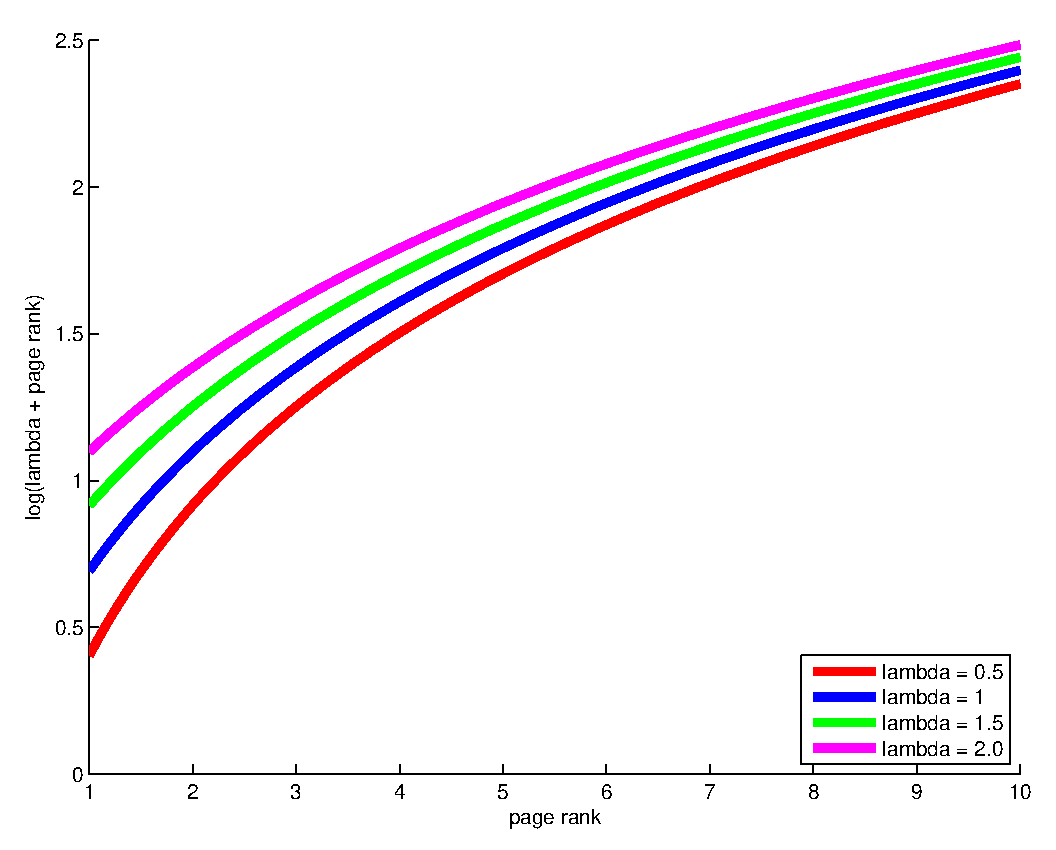
\includegraphics[width=\textwidth]{V_function.eps} \\
  \caption{$V_\textrm{page rank} = \log(\lambda^\prime + \textrm{page rank})$ with different $\lambda^\prime$s}\label{img:logfunction}
\end{center}
\end{figure}
  
  
  \item[] 5. For a function that includes the smallest window as one component, how does varying $B$ and the boost function change the performance of the ranking algorithm?
      
      $B$ has multiplicative effects on the ranking function, where the larger $B$ is, the more impact the smallest window component has on the ranking algorithm.
\end{itemize}

\section{Parameters}
The reported ndcg scores on these three tasks are in Table \ref{tab:ndcg}.
\begin{table}[h!]
\begin{center}
\begin{tabular}{|l|l|}
  \hline
   & NDCG \\
  \hline
  Task 1 & 0.8662 \\
  Task 2 & 0.8758 \\
  Task 3 & 0.8682 \\
  \hline
\end{tabular}
  \caption{NDCG scores}\label{tab:ndcg}
\end{center}
\end{table}

\subsection{Task 1}
\begin{verbatim}
task1_W_title = 1.0
task1_W_header = 0.5
task1_W_url = 0.1
task1_W_body = 0.3
task1_W_anchor = 2.0
\end{verbatim}

\subsection{Task 2}
\begin{verbatim}
task2_W_title = 1.0
task2_W_header = 0.5
task2_W_url = 0.1
task2_W_body = 0.3
task2_W_anchor = 2.0
task2_B_title = 0.3
task2_B_header = 0.5
task2_B_url = 2.0
task2_B_body = 1.0
task2_B_anchor = 0.1
task2_K_1 = 0.8
task2_lambda = 0.5
task2_lambda_prime = 0.5 
\end{verbatim}


\subsection{Task 3}
\begin{verbatim}
task3_W_title = 1.0
task3_W_header = 0.5
task3_W_url = 0.1
task3_W_body = 0.3
task3_W_anchor = 2.0
task3_B = 600.0
\end{verbatim}


\end{document}

